\documentclass[11pt,a4paper]{article}
\usepackage[margin=1in]{geometry}
\usepackage{graphicx}
\usepackage{float}
\usepackage{amsmath}
\usepackage{hyperref}
\usepackage{array}
\usepackage{booktabs}
\graphicspath{{./report_assets/}}
\hypersetup{hidelinks}

\title{Homework 3 Report\\Planning with A* and Dynamic Window Approach}
\author{Intelligent Robotics}
\date{\today}

\begin{document}

\maketitle

\section{Overview}

This report summarizes the implementation and validation results for Homework 3. The assignment contains three parts:

\begin{enumerate}
    \item A* search on a grid map.
    \item Dynamic Window Approach (DWA) for local obstacle avoidance.
    \item A combined planner that uses A* as a global guide and DWA as a local controller.
\end{enumerate}

The main implementation files are:

\begin{itemize}
    \item \texttt{source/Astar.py}
    \item \texttt{source/dwa.py}
    \item \texttt{source/question1\_run.py}
    \item \texttt{source/question2\_run.py}
    \item \texttt{source/question3\_run.py}
\end{itemize}

\section{Method}

\subsection{A* Search}

The A* planner uses the standard evaluation function
\[
f(n) = g(n) + h(n),
\]
where $g(n)$ is the accumulated path cost from the start node to the current node, and $h(n)$ is the heuristic estimate from the current node to the goal.

In this homework, the heuristic is the Euclidean distance:
\[
h(n) = \sqrt{(x_n - x_g)^2 + (y_n - y_g)^2}.
\]

The planner maintains a priority queue for the frontier and stores the parent of each expanded node so that the final path can be reconstructed after reaching the goal.

\subsection{Dynamic Window Approach}

The DWA planner samples admissible velocities in the local dynamic window around the current robot velocity. For each candidate velocity pair $(v_x, v_y)$, the algorithm predicts a short trajectory and evaluates it with a weighted cost:
\[
J = k_v J_v + k_g J_g + k_o J_o + k_a J_a.
\]

The terms are:

\begin{itemize}
    \item $J_v$: velocity cost, which prefers larger speeds.
    \item $J_g$: goal cost, which prefers predicted trajectories that end closer to the goal.
    \item $J_o$: obstacle cost, which penalizes trajectories that pass near obstacles.
    \item $J_a$: A* guidance cost, which is used only in Question 3.
\end{itemize}

Trajectories that collide with obstacles or leave the valid map area are assigned a very large obstacle cost, which effectively removes them from consideration.

\subsection{Combined A* + DWA Planning}

In Question 3, A* first generates a collision-free global path on the grid map. During local motion planning, DWA adds a path-following term based on the distance between the predicted local trajectory and the A* global path. This keeps the robot close to the global route while preserving the reactive obstacle avoidance behavior of DWA.

\section{Results}

\subsection{Question 1: A* Search}

\begin{table}[H]
\centering
\begin{tabular}{@{}ll@{}}
\toprule
Metric & Value \\
\midrule
Visited nodes & 268 \\
Path points & 31 \\
Path length & 3.580 m \\
\bottomrule
\end{tabular}
\caption{Question 1 statistics}
\end{table}

\begin{figure}[H]
\centering
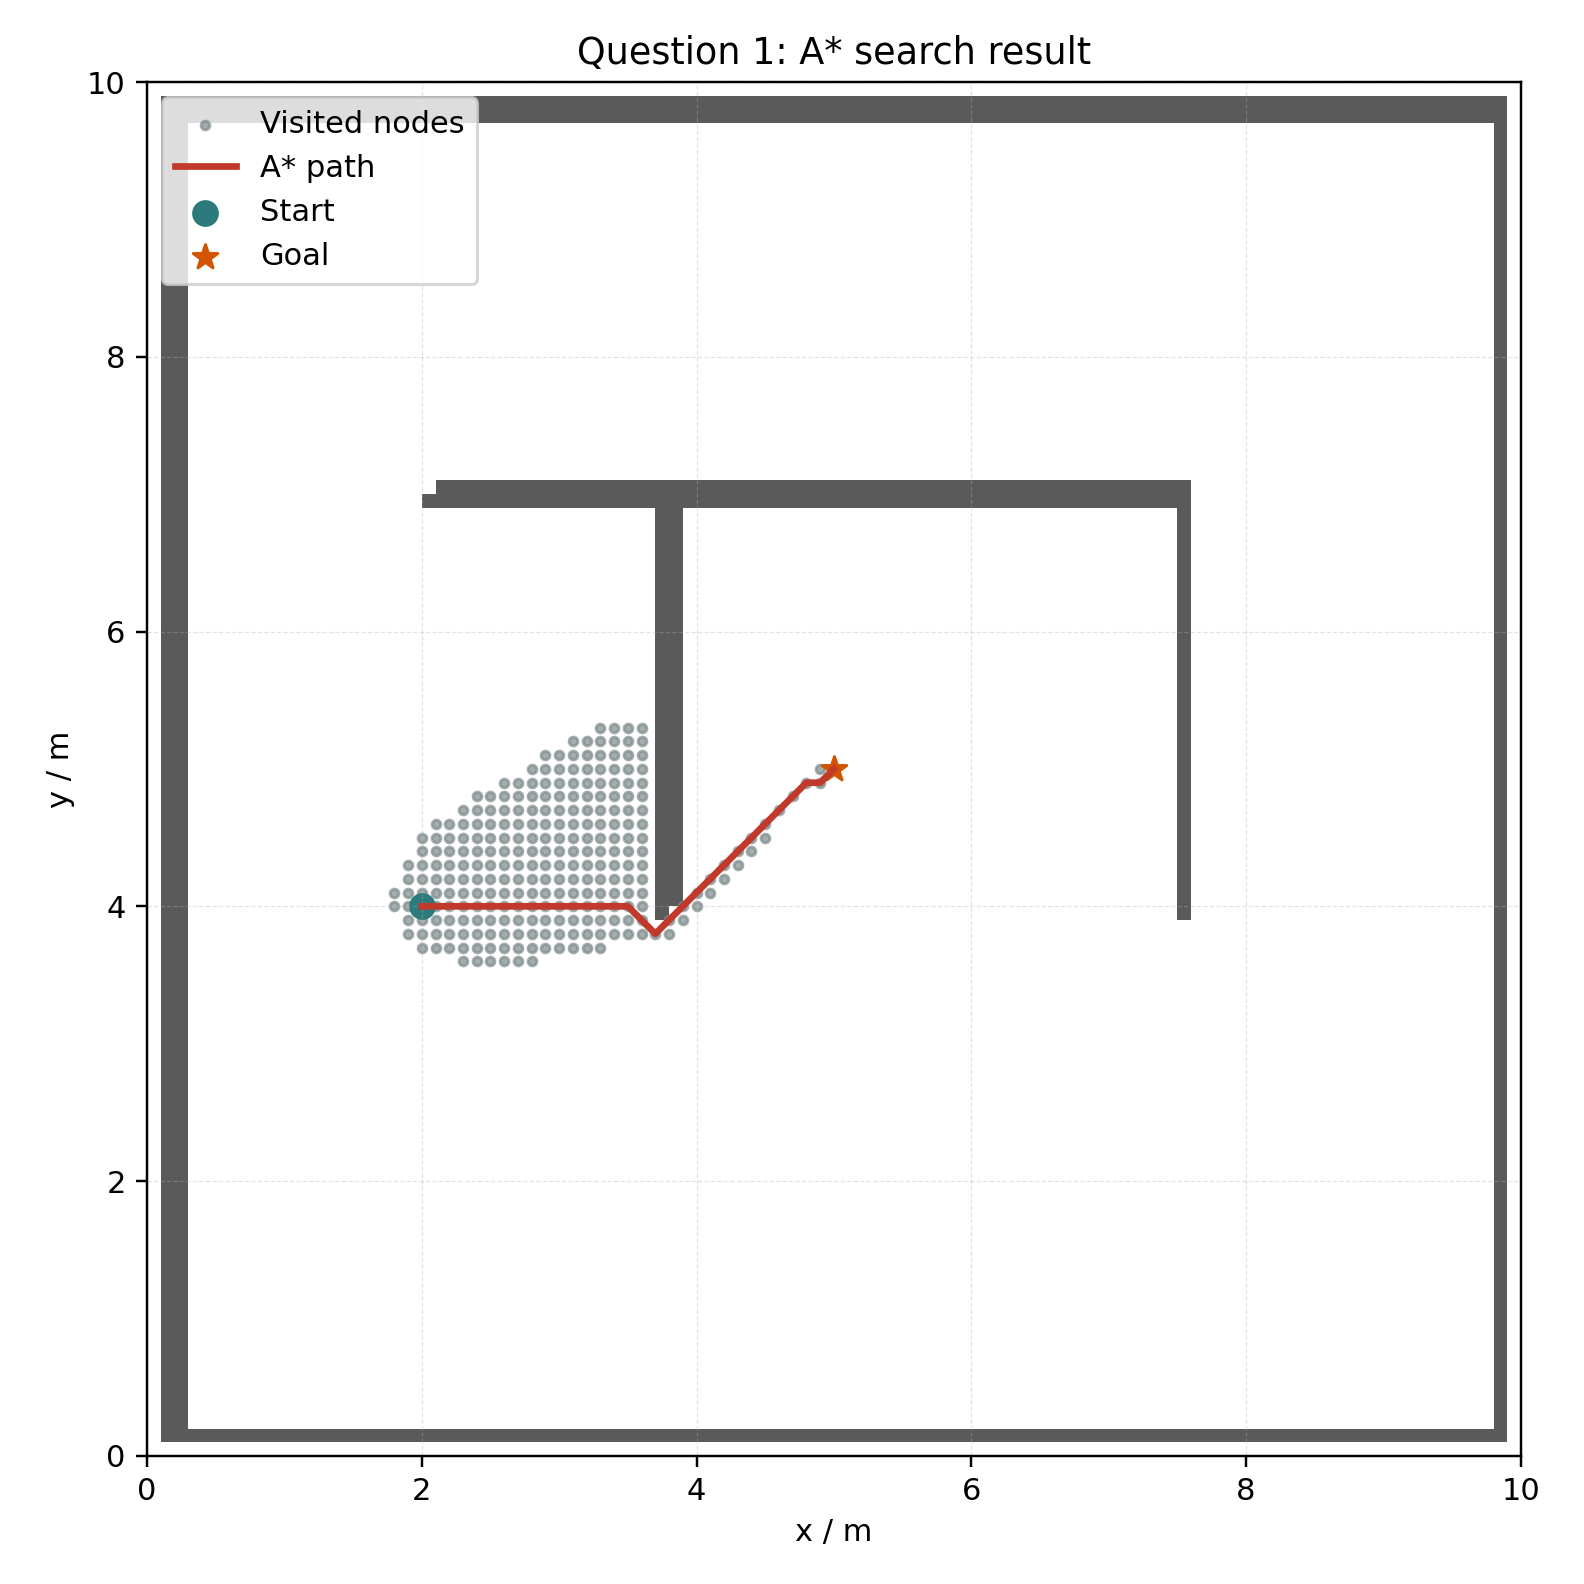
\includegraphics[width=0.78\textwidth]{q1_astar.png}
\caption{Visited nodes and final A* path}
\end{figure}

\subsection{Question 2: DWA}

\begin{table}[H]
\centering
\begin{tabular}{@{}ll@{}}
\toprule
Metric & Value \\
\midrule
Steps to reach goal region & 38 \\
Final distance to goal & 0.170 m \\
Trajectory length & 6.191 m \\
\bottomrule
\end{tabular}
\caption{Question 2 statistics}
\end{table}

\begin{figure}[H]
\centering
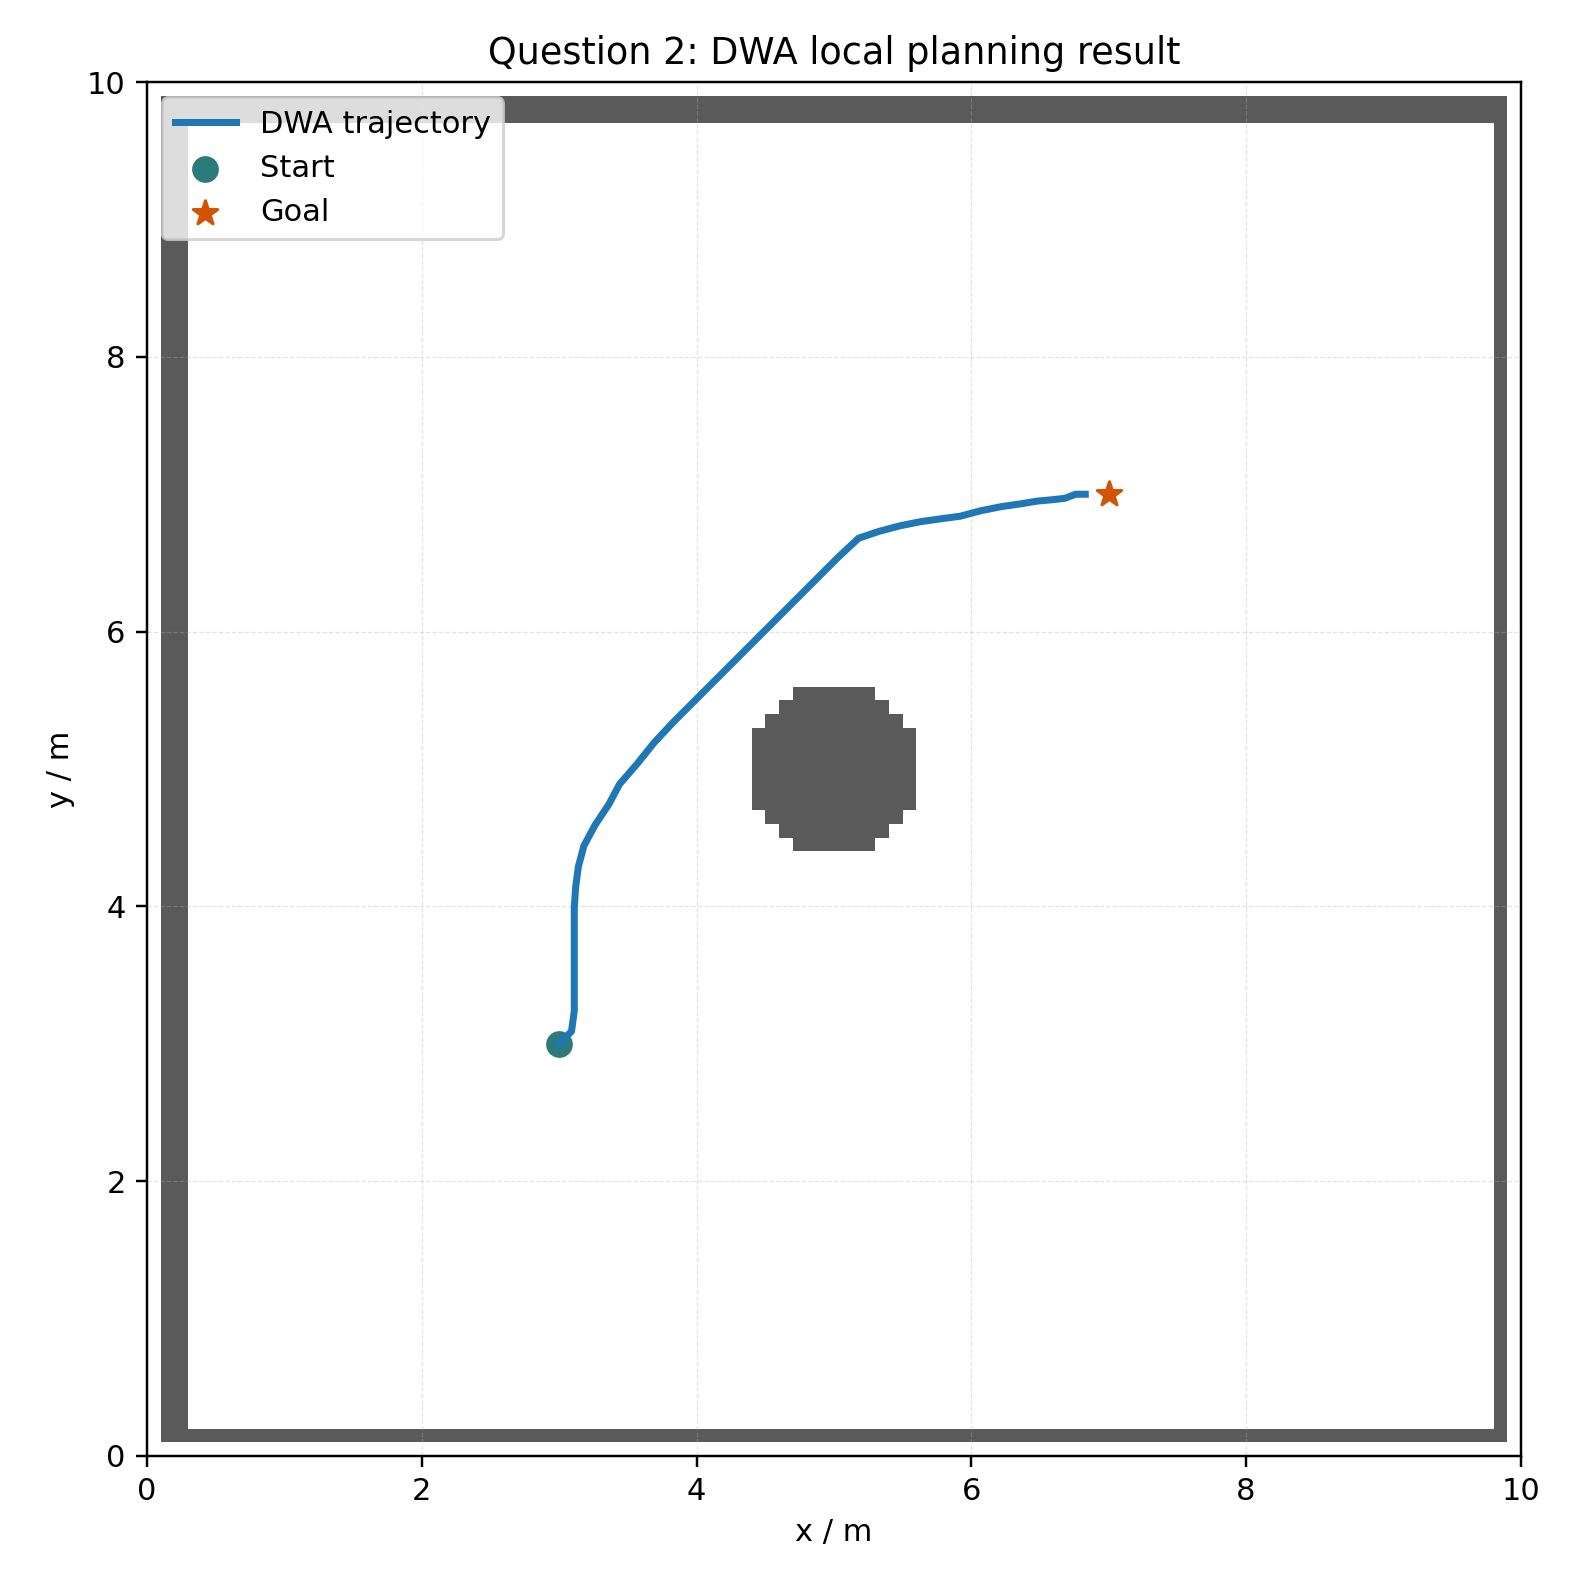
\includegraphics[width=0.78\textwidth]{q2_dwa.png}
\caption{DWA local planning trajectory}
\end{figure}

\subsection{Question 3: A* + DWA}

\begin{table}[H]
\centering
\begin{tabular}{@{}ll@{}}
\toprule
Metric & Value \\
\midrule
A* path points & 31 \\
Steps to reach goal region & 67 \\
Final distance to goal & 0.130 m \\
Trajectory length & 10.839 m \\
\bottomrule
\end{tabular}
\caption{Question 3 statistics}
\end{table}

\begin{figure}[H]
\centering
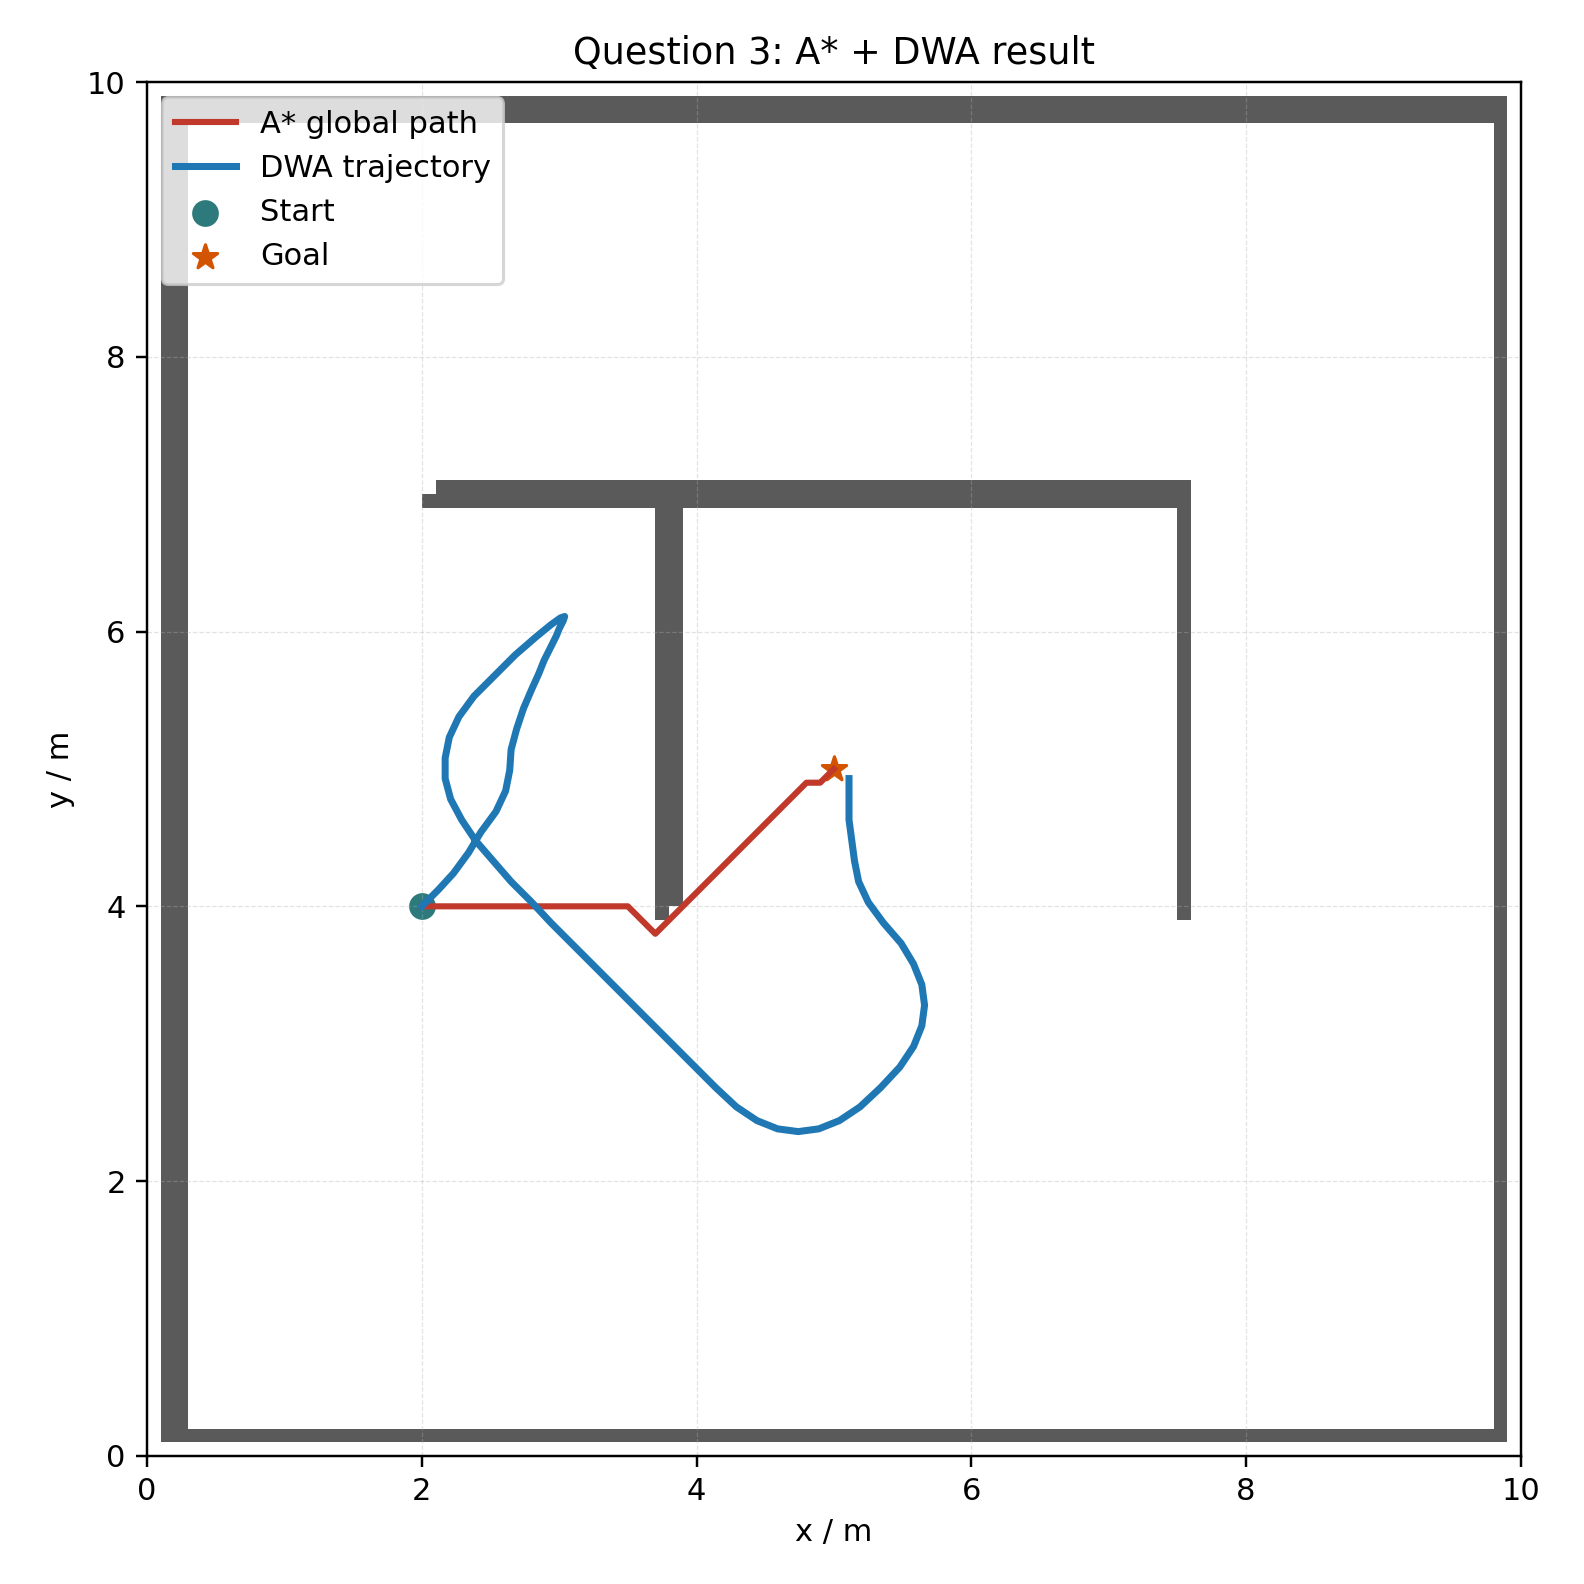
\includegraphics[width=0.78\textwidth]{q3_astar_dwa.png}
\caption{A* global path and DWA executed trajectory}
\end{figure}

\section{How To Run}

Run the three tasks from \texttt{hw3/source}:

\begin{verbatim}
py -3.9 question1_run.py
py -3.9 question2_run.py
py -3.9 question3_run.py
\end{verbatim}

To export animations:

\begin{verbatim}
py -3.9 question1_run.py -a
py -3.9 question2_run.py -a
py -3.9 question3_run.py -a
\end{verbatim}

To rebuild this PDF report from \texttt{hw3}:

\begin{verbatim}
pdflatex report.tex
\end{verbatim}

\section{Conclusion}

The completed homework demonstrates three levels of planning functionality. A* provides a reliable global search method on the occupancy grid, DWA provides reactive local motion generation with obstacle avoidance, and the combined A* + DWA planner shows how a global route and a local controller can work together to guide the robot safely to the goal.

\end{document}
